\section{Numerical Implementation}

The numerical implementation couples conservative DBS transport with
cell-centred PHREEQC chemistry and cell-based surface complexation in a single
operator-split formulation. The discussion below describes the discrete fields,
the transport--chemistry coupling, and the timestep algorithm used in the
reported simulations.

\subsection{Field Locations And Discretization}

The baseline discretization keeps all chemistry-bearing state cell-centered.
This avoids introducing an extra face reconstruction for the unresolved
surface-reaction source. The solution species, $\theta$,
$\epsilon_{\mathrm{num}}$, $a_{\mathrm{surf}}$, and the surface fields are
therefore stored at cell centres, whereas only the volumetric flux $\phi$
remains face-centred. Transport uses face interpolation only within the
conservative flux assembly, while the surface chemistry remains strictly
cell-local.

For microporous image cases, the current implementation treats the cell-centered
surface-area field as an additive quantity:
\[
    a_{\mathrm{surf}} =
    a_{\mathrm{surf}}^{\mathrm{interface}} +
    a_{\mathrm{surf}}^{\mathrm{intrinsic}}.
\]
The first term is the coarse-grained phase-boundary contribution. The second is
an intrinsic volumetric surface density assigned to selected image phases
(for example the micropore phase) and scaled by the corresponding local phase
fraction inside each coarse cell.

\subsection{PHREEQC Coupling}

The PHREEQC coupling is performed through \texttt{phreeqcDBSMixture}. For each
cell, the coupling uses the current aqueous state, the physical mobile-water
fraction $\theta$, the current cell surface area $a_{\mathrm{surf}}$ including
any intrinsic micropore contribution, and the current cell surface state. The
surface mode is optional and reduces exactly to aqueous-only mode when
$a_{\mathrm{surf}} = 0$.

Cells with negligible mobile-water fraction remain chemically inactive in the
written finite-volume state. In the current implementation this is enforced at
the field level, even though the PHREEQC backend may still use an internal
dummy water volume to keep the chemistry module numerically well-posed.

\subsection{Per-Timestep Algorithm}

The production timestep is intentionally simple. At each step, the solver reads
or updates the face flux $\phi$, advances each aqueous transport equation in
conservative DBS form, pushes the updated cell state into PHREEQC, executes
the local chemistry update, pulls the updated aqueous and surface states back
into the finite-volume fields, and finally writes diagnostics, including
integrated inventory summaries. This is the appropriate baseline for a first
conservative implementation because the transport and chemistry operators
remain individually testable.

\begin{figure}[htbp]
    \centering
    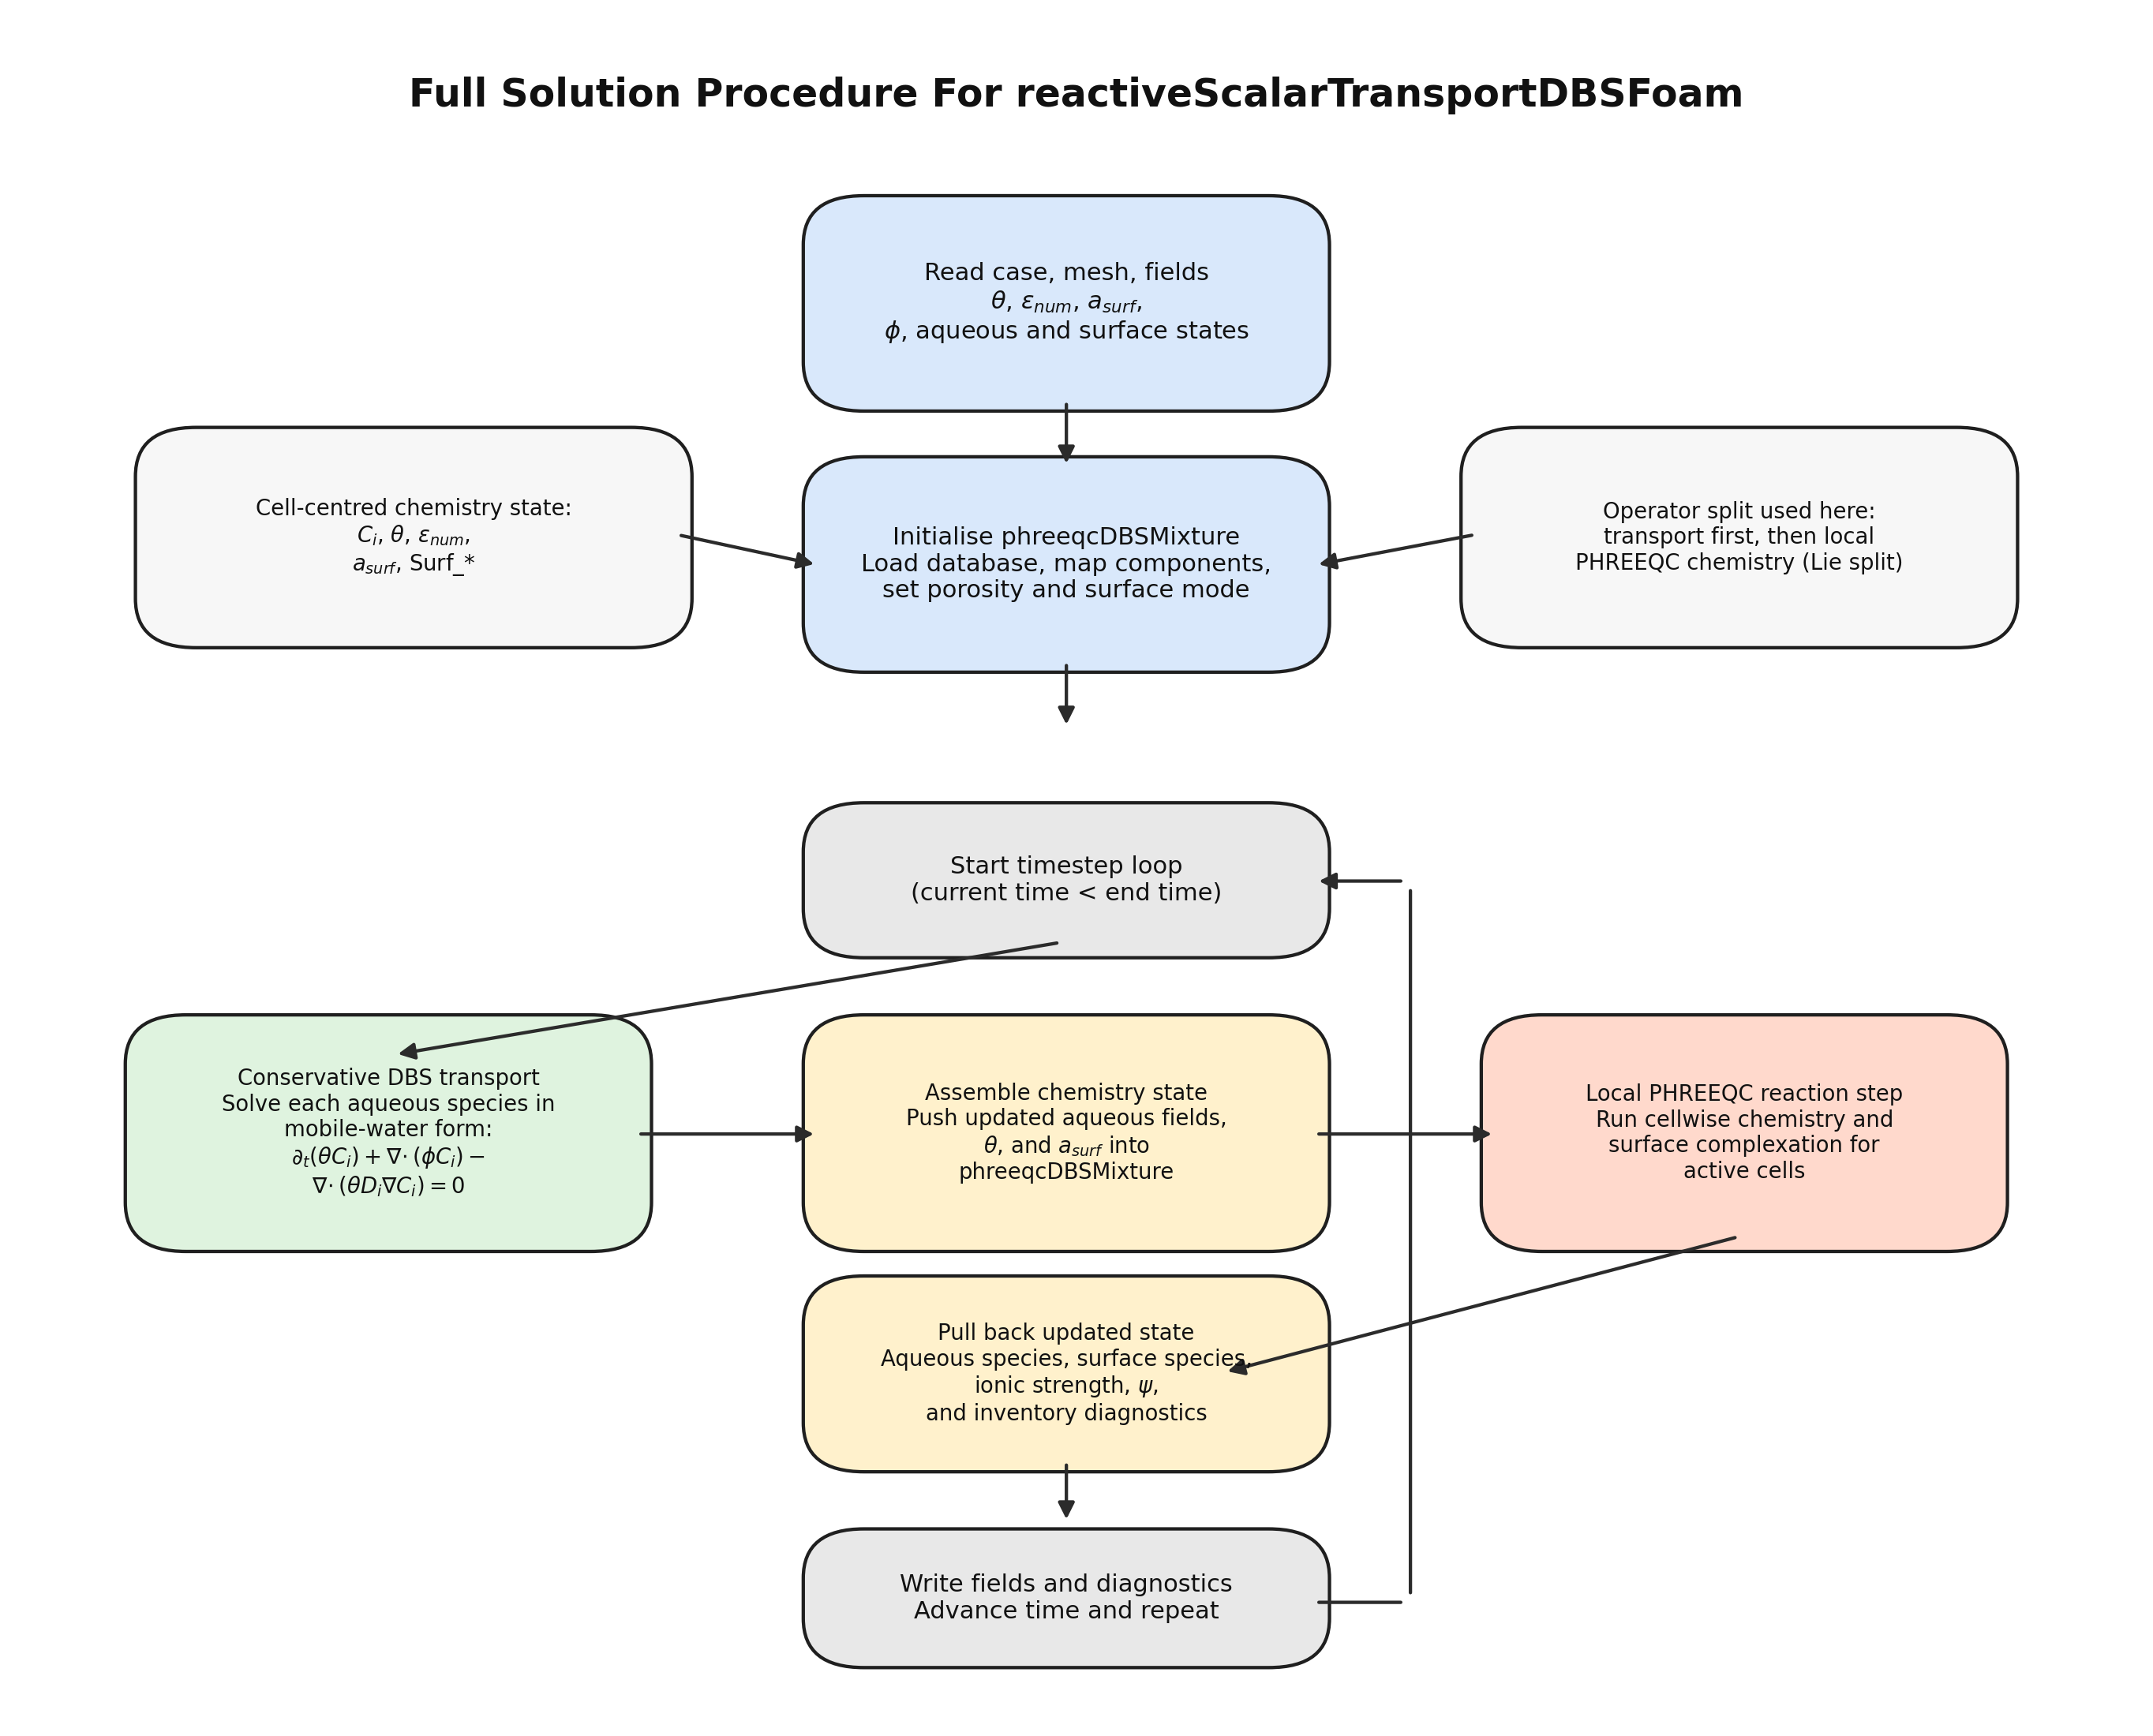
\includegraphics[width=0.96\linewidth]{figures/png/fig05_solver_workflow.png}
    \caption{Full solution procedure for
    \texttt{reactiveScalarTransportDBSFoam}. The solver reads the current
    finite-volume state, initializes or updates the cell-based PHREEQC
    coupling through \texttt{phreeqcDBSMixture}, advances all aqueous species
    in conservative DBS form, executes the local cellwise chemistry update,
    and then writes the updated aqueous and surface states back to the
    finite-volume fields. The workflow is intentionally operator-split:
    transport is solved first, followed by local PHREEQC chemistry, so the two
    operators remain independently testable and the conservative structure of
    the aqueous transport step is never hidden inside an implicit composite
    source term.}
    \label{fig:dbsWorkflow}
\end{figure}

Figure~\ref{fig:dbsWorkflow} states the implemented algorithm explicitly. The
key point for the present formulation is that the chemistry state remains
cell-centred throughout the loop. The solver does not reconstruct a face-based
reaction source for the unresolved surface term. Instead, the transport
operator acts on cell inventories through the face fluxes, while the reaction
operator acts locally on the updated cell state through PHREEQC.

\subsection{Current Operating Limits}

The present operating limits should be stated explicitly. Local decomposition
sensitivity on very small benchmark meshes is not at write precision, and
small timestep or mesh refinements can still alter the local front shape by a
few percent on the fixed 1D benchmark. In addition, the written DBS surface
fields follow the inherited field-scaling convention documented in the
implementation notes. For microporous image cases, the intrinsic micropore
surface density remains a case input rather than a quantity inferred uniquely
from the segmented image. Finally, exact surface-state restart is not yet a
fully validated capability for the upgraded backend because saved
\texttt{Surf\_*} fields are not reintroduced into PHREEQC exactly; the
surface-enabled production results reported here therefore rely on clean
starts.
